%%%%%%%%%%%%%%%%%%%%%%%%%%%%%%%%%%%%%%%%%%%%%%%%%%%%%%%%%%%%%%%%%%%%%
%% This is a (brief) model paper using the achemso class
%% The document class accepts keyval options, which should include
%% the target journal and optionally the macuscript tye
%%%%%%%%%%%%%%%%%%%%%%%%%%%%%%%%%%%%%%%%%%%%%%%%%%%%%%%%%%%%%%%%%%%%%
\documentclass[journal=jacsat,manuscript=article]{achemso}

%%%%%%%%%%%%%%%%%%%%%%%%%%%%%%%%%%%%%%%%%%%%%%%%%%%%%%%%%%%%%%%%%%%%%
%% Place any additional packages needed here.  Only include packages
%% which are essential, to avoid problems later.
%%%%%%%%%%%%%%%%%%%%%%%%%%%%%%%%%%%%%%%%%%%%%%%%%%%%%%%%%%%%%%%%%%%%%
\usepackage[version=3]{mhchem} % Formula subscripts using \ce{}
\usepackage{graphicx}

%%%%%%%%%%%%%%%%%%%%%%%%%%%%%%%%%%%%%%%%%%%%%%%%%%%%%%%%%%%%%%%%%%%%%
%% If issues arise when submitting your manuscript, you may want to
%% un-comment the next line.  This provides information on the
%% version of every file you have used.
%%%%%%%%%%%%%%%%%%%%%%%%%%%%%%%%%%%%%%%%%%%%%%%%%%%%%%%%%%%%%%%%%%%%%
%%\listfiles

%%%%%%%%%%%%%%%%%%%%%%%%%%%%%%%%%%%%%%%%%%%%%%%%%%%%%%%%%%%%%%%%%%%%%
%% Place any additional macros here.  Please use \newcommand* where
%% possible, and avoid layout changing macros (which are not used
%% when typesetting).
%%%%%%%%%%%%%%%%%%%%%%%%%%%%%%%%%%%%%%%%%%%%%%%%%%%%%%%%%%%%%%%%%%%%%
\newcommand*{\mycommand}[1]{\texttt{\emph{#1}}}

%%%%%%%%%%%%%%%%%%%%%%%%%%%%%%%%%%%%%%%%%%%%%%%%%%%%%%%%%%%%%%%%%%%%%
%% Meta-data block
%% ---------------
%% Each author should be given as a separate \author command.
%%
%% Corresponding authors should have an e-mail given after the author
%% name as an \email command.
%%
%% The affiliation of authors is given after the authors; each
%% \affiliation command applies to all preceding authors not already
%% assigned an affiliation.
%%
%% The affiliation takes an option argument for the short name.  This
%% will typically be something like "University of Somewhere".
%%
%% The \altaffiliation macro should be used for new address, etc.
%%%%%%%%%%%%%%%%%%%%%%%%%%%%%%%%%%%%%%%%%%%%%%%%%%%%%%%%%%%%%%%%%%%%%
\author{Robert Jensen}
\author{Thomas Andersen}
\author{Anders Nierhoff}
\affiliation{CINF, Department of Physics, Technical University of Denmark, Fysikvej 312, 2800 Lyngby, Denmark.}
\author{Thomas Pedersen}
\author{Ole Hansen}
\affiliation{CINF, Department of Micro- and Nanotechnology, Technical University of Denmark, \O rsteds Plads, B 345B, 2800 Lyngby, Denmark.}
\author{S\o ren Dahl}
\author{Ib Chorkendorff}
\email{ibchork@fysik.dtu.dk}
\affiliation{CINF, Department of Physics, Technical University of Denmark, Fysikvej 312, 2800 Lyngby, Denmark.}

%%%%%%%%%%%%%%%%%%%%%%%%%%%%%%%%%%%%%%%%%%%%%%%%%%%%%%%%%%%%%%%%%%%%%
%% The document title should be given as usual
%% A short title can be given as a *suggestion* for running headers.
%%%%%%%%%%%%%%%%%%%%%%%%%%%%%%%%%%%%%%%%%%%%%%%%%%%%%%%%%%%%%%%%%%%%%
\title[Oxidation oscillations at atmospheric pressure]
{Self-sustained carbon monoxide oxidation oscillations on size-selected platinum nanoparticles at atmospheric pressure}

\begin{document}
%%%%%%%%%%%%%%%%%%%%%%%%%%%%%%%%%%%%%%%%%%%%%%%%%%%%%%%%%%%%%%%%%%%%%
%% The manuscript does not need to include \maketitle, which is
%% executed automatically.  The document should begin with an
%% abstract, if appropriate.  If one is given and should not be, the
%% contents will be gobbled.
%%%%%%%%%%%%%%%%%%%%%%%%%%%%%%%%%%%%%%%%%%%%%%%%%%%%%%%%%%%%%%%%%%%%%
\begin{abstract}
  High-quality mass spectrometry data of the oscillatory behavior
  of CO oxidation on SiO$_2$ supported Pt-nanoparticles at atmospheric
  pressure has been acquired as a function of pressure, coverage, gas
  composition and nanoparticle size. The oscillations are self-sustained
  for several days at constant temperature, pressure and CO/O$_2$ ratio.
  The frequency of the oscillations is very well defined and increases
  over time. The oscillation frequency is furthermore strongly temperature
  dependent with increasing temperature resulting in increasing frequency.
  A plausible mechanism for the oscillations is proposed based on a
  oxidation/reduction cycle of the nanoparticles which change the rate of
  CO oxidation on the particles.
\end{abstract}

%%%%%%%%%%%%%%%%%%%%%%%%%%%%%%%%%%%%%%%%%%%%%%%%%%%%%%%%%%%%%%%%%%%%%
%% Start the main part of the manuscript here.
%%%%%%%%%%%%%%%%%%%%%%%%%%%%%%%%%%%%%%%%%%%%%%%%%%%%%%%%%%%%%%%%%%%%%
\section{Introduction}

Self-sustained oscillating systems are wide spread in nature and have been
described both experimentally and theoretically. One of the maybe most famous
biological examples is the oscillation in the lynx-hare population as
reported through the number furs delivered to the Hudson Bay Company A).
This was for some time was believed to be forced by the sunspot oscillations,
however, this proved to be a coincidence B) and could be described alone
by a close dynamical coupling in between the two populations. Similar very
interesting observations have been made for our current climate changes
\cite{Svensmark1997,Svensmark1998} suggesting that the sunspot activity could
influences the level of cosmic rays and thus the cloud formation, but this
currently a topic of controversy \cite{Lockwood2007}. A beautiful example of
self-sustained oscillatory behavior in chemistry is the colorful
Belousov-Zhabotinsky reaction which is rather easy to demonstrate for an
audience\cite{ZAIKIN1970}. Such self-sustained oscillatory behavior has been
explained for systems far from equilibrium in several theoretical works
\cite{HakenBog,NicolisBog}. Similar behavior has been observed within
heterogeneous catalysis where typically nanoparticles of a precious metal
supported on an inexpensive oxide constitute the active phase \cite{IbsBog}.
One of the very first examples was observed by Wicke for CO oxidation on a
catalyst of highly dispersed Pt on γ−Al2O3 \cite{BEUSCH1972}. To gain a deeper
insight into the fundamental aspects of such oscillatory reactions this work
was followed up by Ertl on Pt(110) surfaces under well-defined conditions
\cite{EISWIRTH1986}. Ertl demonstrated how the switching in between the
unreconstructed Pt(110) surface and the reconstruction 2x1-Pt(110) surface
combined with big changes of oxygen sticking coefficient on the two surfaces
could drive the self-sustained oscillations. This and many other interesting
aspects of self-sustained and forced oscillatory behavior and spatio–temporal
self-organization were investigated by Ertl and coworkers on well-defined
single crystals see for example reviews \cite{IMBIHL1995,JAKUBITH1990} and in
particular the Nobel Lecture \cite{Ertl2008}. One of the reasons this has
attracted so much interest is naturally the importance of such catalytic
reactions and therefore a demand to gain a better understanding of their
behavior with the goal of further improvement. CO oxidation is one of the most
studied reactions due to its importance in both automotive catalysis and in
the removal of trace CO in hydrogen streams \cite{IbsBog}. The oscillatory
behavior is, however, limited to either Pt or the CO oxidation, but
have been found for many other metallic catalyst like on for example Rh, Ir,
and Pd and for oxidations reactions in general as well as for NO and CO
reactions and even for hydrogenation reactions \cite{Lund2000,SALES1982}. Most
of the studies are made on single crystal or poly crystalline films or
filaments, mainly in conjunction with ultra-high vacuum equipment so that the
surfaces can be characterized using the surface science methods. The amount of
work described on supported catalyst seems more limited obviously because it
is so much more difficult to characterize those systems and because additional
complexities are present such as mass and heat transport. There even exist
reports in the literature of how large scale facilities such as an industrial
ammonia fixed-bed synthesis reactor in Germany in 1989 started oscillating for
several hours. This could be modeled by a coupling of the exothermic process
and the heat management in the reactor system \cite{Machado2005}, but one
cannot rule out that the observed oscillations could in some systems also be
created by inherent processes on the catalyst itself. In general such
oscillations would be considered highly undesirable in industry since they
could be difficult to control and result in run-away incidents in particular
for exothermic reactions resulting in damaged catalyst due to sintering at
higher temperatures. On the other hand there exist examples in the literature
where forced oscillations seem to improve the overall activity
\cite{IMBIHL1995,Machado2005} . One particular interesting process here could
be the methanol synthesis where reducing the CO$_2$ contents for a shorter period
of time result in a subsequent higher methanol rate over compensation for the
lack of methanol production when running in the reducing H$_2$ and CO alone
\cite{Dynamics-Bog}. This enhancement can be explained by extensive wetting
and un-wetting of the active Copper catalyst dependent on the oxidation
potential \cite{Hansen2002} i.e. the active area is strongly increased when
reduced but slowly returns to the less active state when the CO$_2$ is present.

As mentioned the understanding of self-sustained on supported catalyst is
hampered by the fact that entirely different mechanism than those observed on
single and polycrystalline samples may exist. For example on a Pt(110) crystal
it was shown how waves of surface reconstruction could propagate on the
surface ensuring a synchronization of the phenomena. This also have to occur
for oscillation on supported catalyst, but here it is more likely to be due to
coupling of mass or heat transport. There have been a few examples where such
oscillations have been observed. Of these are the most prominent the work by
Skoghlund \cite{Carlsson2006} where self-sustained oscillations were observed
on supported Pt catalyst and simultaneous studied by in situ IR spectrometry.
Similar studies were recently undertaken using EXAFS \cite{Singh2010} but here
the oscillatory behavior was rather unstable and somewhat less convincible.

In this work we demonstrate how a two-dimensional model system of Pt
nanoparticles on a SiO2 support can be constructed that displays highly
repeatable self-sustained oscillations when first started. The system consist
of mass selected Pt nanoparticles in the range from 2 to 10\,nm Pt
nanoparticles deposited in a microreactor with a surface area of 0.75\,cm$^2$
specially designed to achieve high sensitivity \cite{Henriksen2009}. This
method offers some advantages over the chemical synthesis methods, which also
offers the possibility of size selected nanoparticles se for example 
\cite{Tsang2008,Shao2011}, since in this case we do not have to bother with
the surfactants required for these synthesis methods. The coverage of Pt
nanoparticles could be varied from sub-percent to full coverage. It is
demonstrated how the nanoparticles could provide self-sustained oscillations
over extend of days and how various parameters could be mapped out inclusive
the influence of the temperature dependence - an effect that could not be
demonstrated for a continuous film of same area and similar conditions. By
combining these results with previous studies \cite{Carlsson2006,Singh2010}
and a recent detailed study of CO oxidation on Pd using STM
\cite{Hendriksen2010} a plausible explanation of the oscillatory behaviors
presented. The low coverage and extremely efficient Pt nanoparticles
illuminates some of the pit falls that may have to be considered when making
in situ investigations of such a system since extremely low coverages may
provide the entire conversion.

A) D. A. McLulich, Variations in the Number of Varying Hare,University of Toronto
Press, Toronto, 1937. (we need to dig in for the correct ref here),
B) I remember reading of this in a biology book back in the seventies, check)

\section{Experimental Methods}
\subsection{The $\mu$-reactor platform}
The experiments were performed in Si-based $\mu$-reactors\cite{Henriksen2009}. The reactor design makes sure that all gases exposed to the catalyst under investigation is measured by the quadropole mass spectrometer (QMS) ensuring an extremely high sensitivity of the system. 

The experiments were performed in Si-based 20x16\,mm $\mu$-reactors\cite{Henriksen2009}. The reactor consists of two inlets, a mixing zone allowing for diffusional mixing of reactants, an outlet, a reactor volume of $240\,$nL and a $5.4\,\mu$m wide, 3\,$\mu$m high and 1500\,$\mu$m long capillary used for sniffing gases from the reactor volume. The reactor is sealed by anodic bonding of a pyrex lid to the Si reactor and is able to operate in a pressure range of 0-2.5\,bar. The reaction gases are supplied to the two inlets by flow controllers capable of controlling the gas flow from 0-10 mL/min. The capillary flow is fed into a quadropole mass-spectrometer (QMS) for analysis while any surplus of gas from the inlets is passed directly through to the outlet via a pressure controller allowing control of reactor pressure. The design makes sure that all gases exposed to the catalyst under investigation are measured by the QMS ensuring an extremely high sensitivity of the system. 

\begin{scheme}
  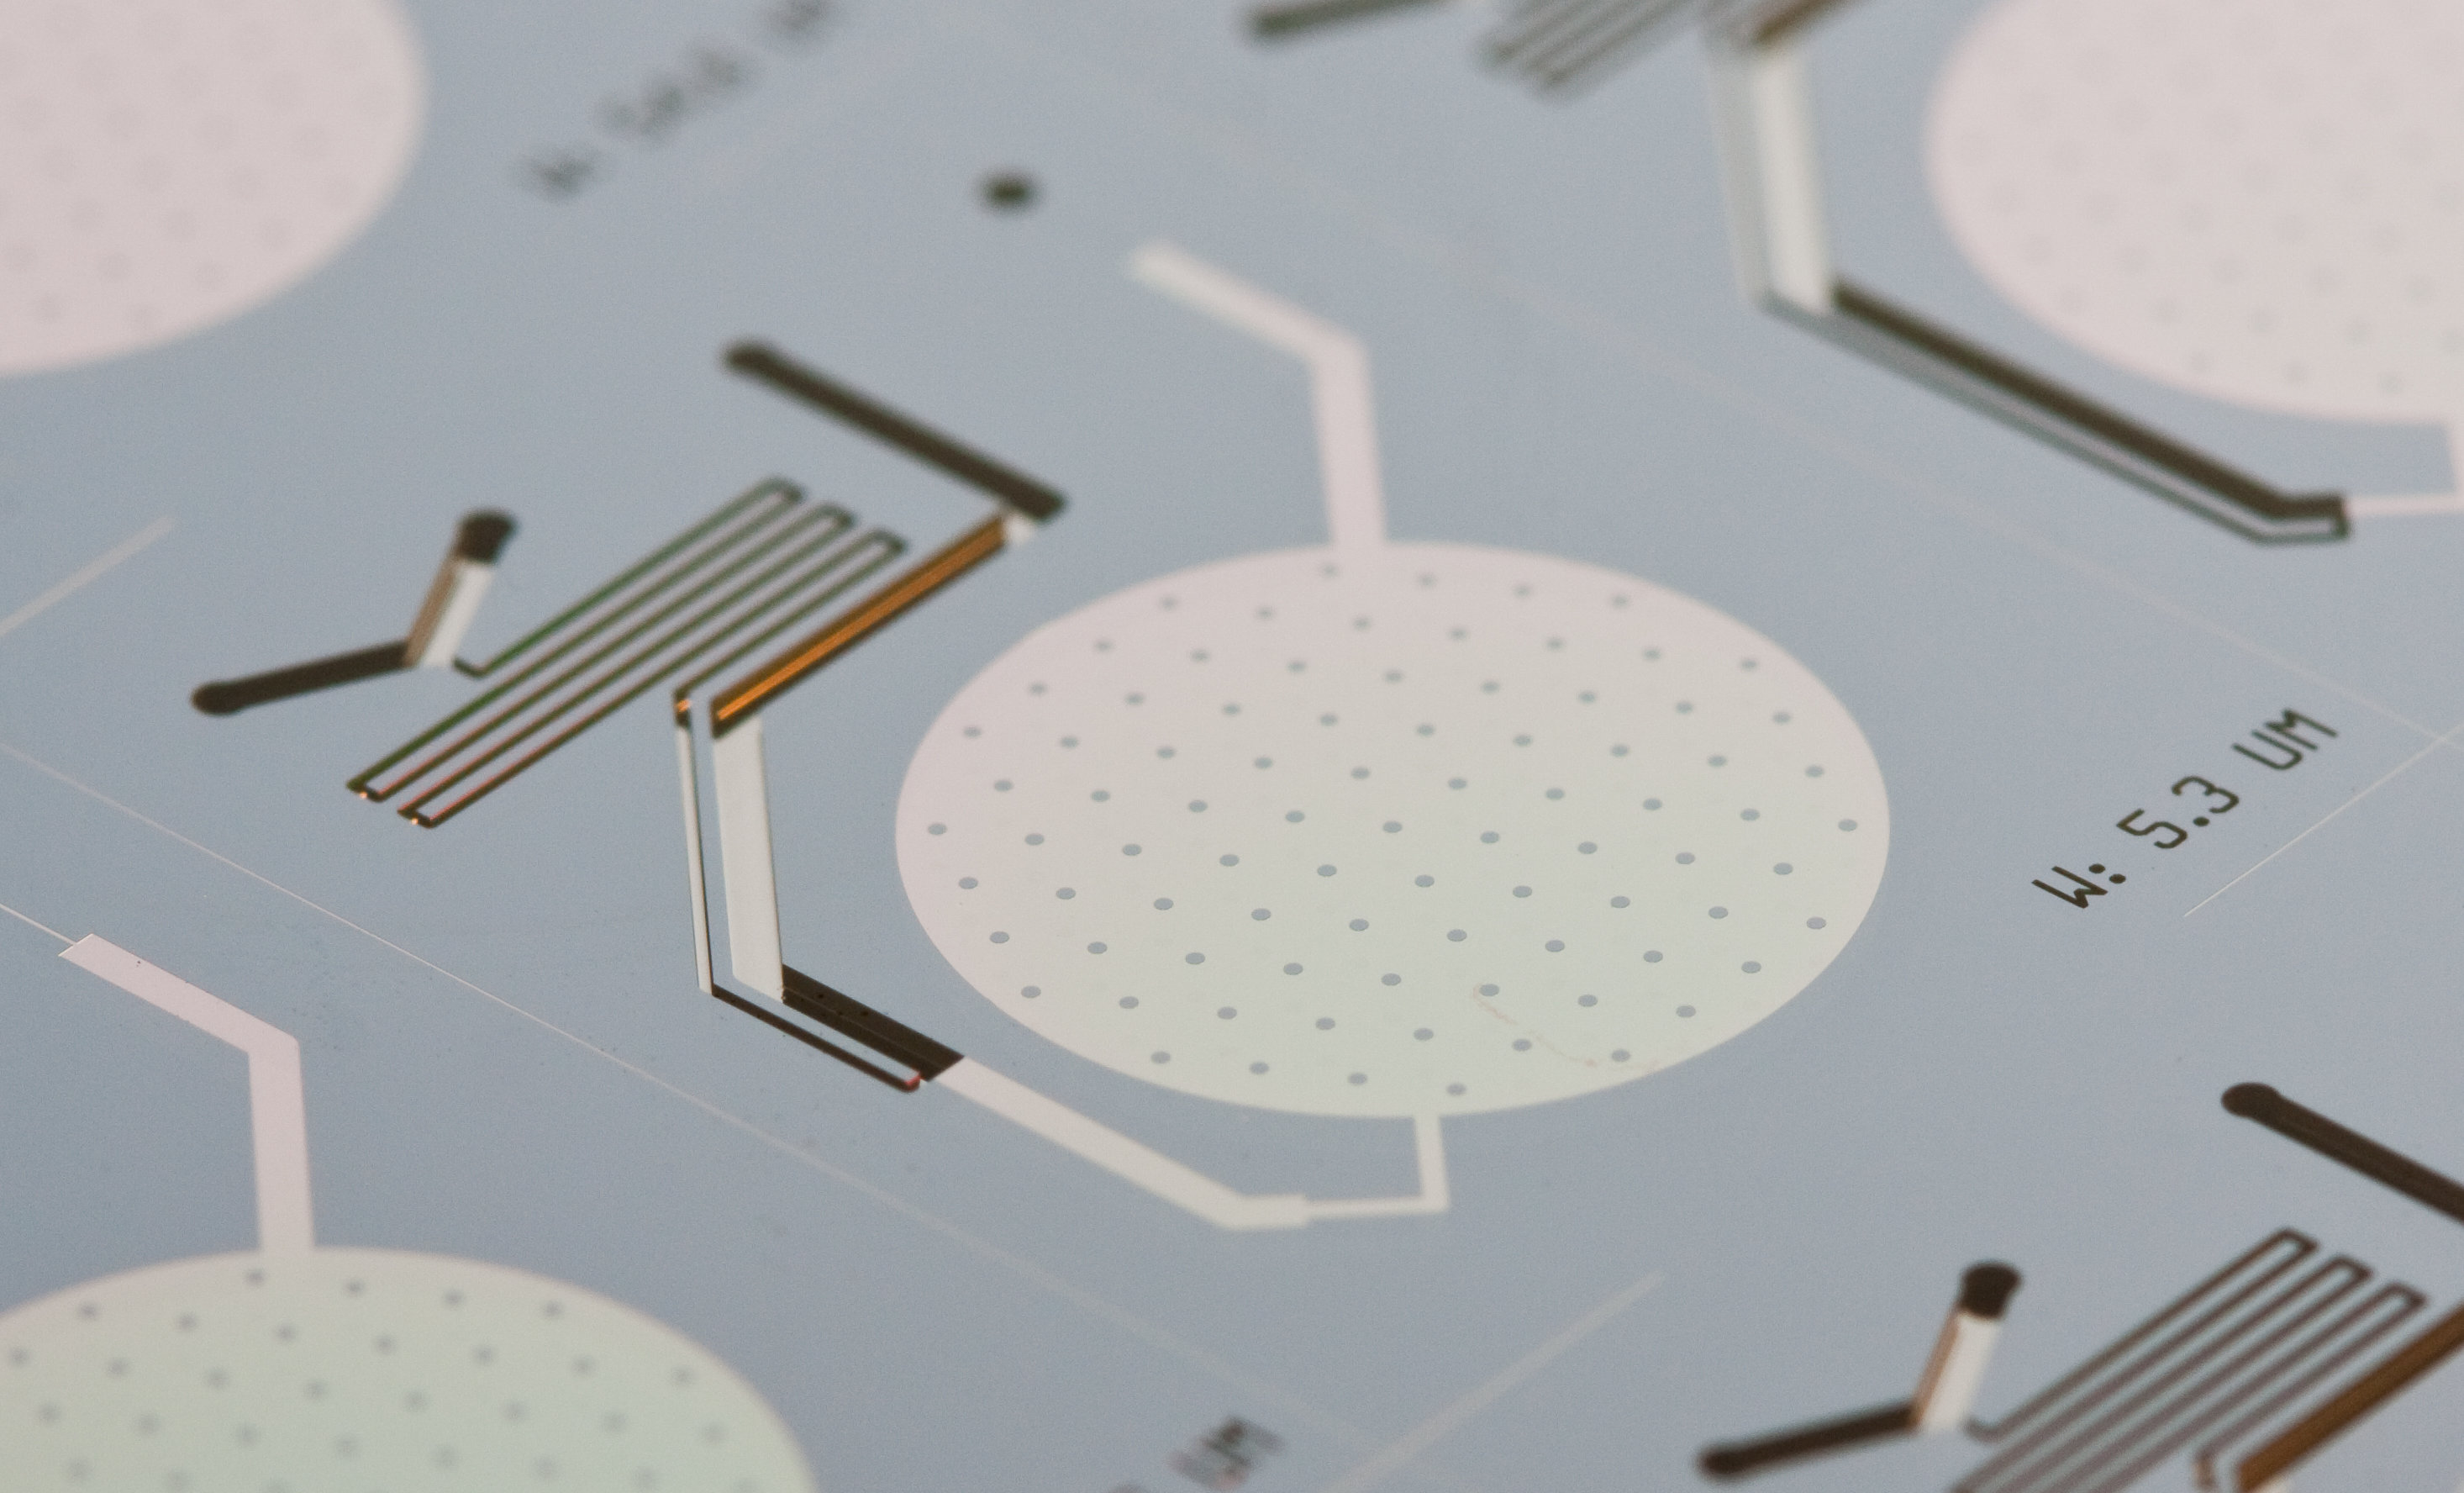
\includegraphics[width=8cm]{reactor.jpg}
  \caption{Image of the 20x16\,mm microreactor showing the circular reactor area and gas channel system}
  \label{fgr:reactor}
\end{scheme}


Before any measurements are performed the reactor is pumped by a turbopump to minimize contaminants in the system. When an evacuated reactor is mounted the base pressure of the mass spectrometer chamber is $\sim5\times10^{-9}\,$mbar and in operation at $1\,$bar in the reactor volume the pressure is $\sim5\times10^{-7}\,$mbar in the QMS chamber. 

The reactor is heated by joule heating of a Pt strip evaporated on the backside of the reactor chip. The introduction of two additional contacts on the backside of the reactor allows for 4 wire measurements of the resistance of the Pt strip using it as a RTD for temperature measurement of the reactor. An external thermocouple acts as room-temperature calibration of the RTD as well as sanity check of the RTD measurement during operation. The measured RTD temperature is always compared to the thermocouple at room temperature both before and after an experiment to be sure the RTD did not change resistance due to annealing during the experiment.

The gas handling including flow and pressure controllers and the mass spectrometer is fully automated allowing for measurements during several days without human intervention allowing for self-consistent measurements of many samples.

\subsection{Pt nanoparticle deposition}
Pt nanoparticles were deposited in the reactor using a gas-aggregation source (Mantis Deposition Ltd., Nanogen 50). Pt clusters were formed by gas-phase condensation of Pt atoms produced by impinging argon ions on a 99.99\% Pt target in a magnetron sputter source. After condensation the ionised fraction (60-80\%) of the clusters were size-selected by a quadropole mass selection filter according to their mass-to-charge ratio. Using this setup Pt nanoparticles with diameters in the range of 2--16\,nm can be produced \cite{Nielsen2010,Nielsen2009}. The size-selected nanoparticles were after size-selection soft-landed in the reactor volume of the microreactor. The coverage was kept at approximately 0.1\% geometric coverage determined by measuring the current on the reactor during deposition. After deposition the reactors were anodically cold-bonded \cite{Vesborg2010} to a pyrex lid to avoid sintering of the nanoparticles while bonding.

\section{Results}
An oscillation measurement is performed by mounting a sample in the setup directly after cluster deposition and anodic bonding. Initially a light-off CO-oxidation measurement is performed (shown in Figure~\ref{fgr:initial_treatment}) where the temperature is increased at 3\,$^\circ$C/min until the sample ignites and achieves full conversion of CO to CO$_2$. At CO:O$_2$ ratio of $\sim0.08$ and a geometrical Pt coverage of $\sim0.1\%$ light-off occurs at approximately 180\,$^\circ$C. The temperature ramp is typically continued up to 260\,$^\circ$C whereafter the temperature is decreased at the same rate as the heating ramp. After the initial light-off the sample is cooled to room temperature. When at room temperature the temperature is again increased at 3\,$^\circ$C/min until sustained oscillations occur. A typical initial treatment is seen in Figure~\ref{fgr:initial_treatment} where both the symmetrical light-off ramp and the subsequent increase in temperature to achieve sustained oscillations is seen. Often the sample will show oscillations either directly upon light-off or on the falling temperature ramp.

\begin{scheme}
  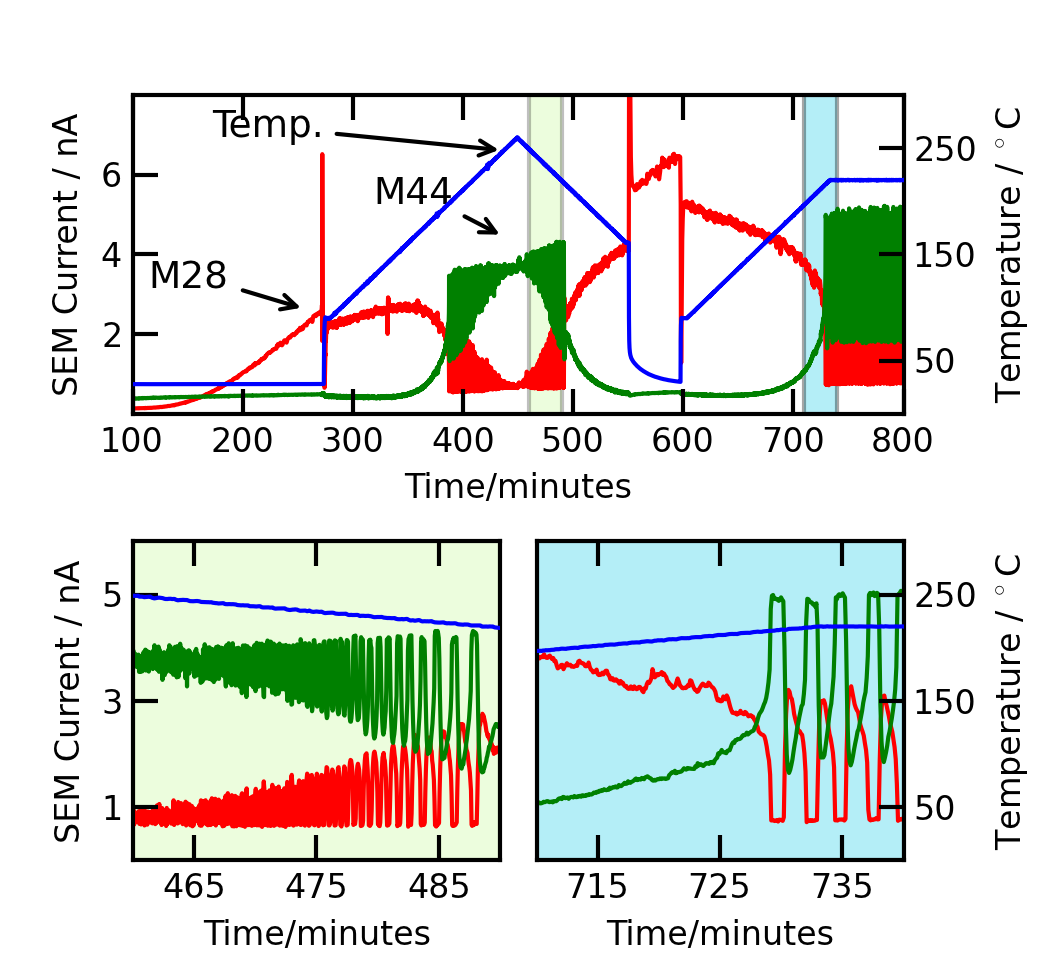
\includegraphics[width=9cm]{initial_treatment.png}
  \caption{A typical example of the initial treatment of a new sample. After performing a light-off ramp where oscillations can been seen the temperature is increased to a constant value where sustained oscillations take place. The non-zero value of CO during high conversion periods is consistent with the expected QMS background signals from CO$_2$ and O$_2$.}
  \label{fgr:initial_treatment}
\end{scheme}

Nanoparticles with sizes ranging from 3\,nm to 9\,nm have been tested but 3\,nm particles with a geometrical coverage of 0.1\% of the reactor area gave the most stable oscillations. No consistent dependency on oscillation frequency and duty cycle was found that could be attributed to the size of the particles.

The oscillations on all samples are qualitatively similar but the oscillation period varies from a few seconds (the time-constant of the reactor is $\sim7\,$s) up to more than an hour. Once a sample start to oscillate it will perform self-sustained oscillations for as long as the experiment is allowed to run. We have not observed a single sample stop oscillating once the self-sustained oscillations had started. 

An example of a single very slow oscillation is seen in Figure~\ref{fgr:full_oscillation}. After a short on-cycle (at $\sim$1030\,min) where all CO is converted to CO$_2$ (notice the CO signal does not go to zero due to the cracking pattern of CO$_2$ and CO background in the QMS) the reaction shows a fast deactivation. After the deactivation the sample quickly regains $\sim$30\% conversion (at $\sim$1040\,min). Hereafter the conversion increases slowly over time until approximately 50\% conversion is reached (at $\sim$1118\,min). Shortly after reaching 50\% conversion the sample again ignites and convert all CO to CO$_2$. After a short full conversion period the sample again deactivates and the cycle repeats itself.

\begin{scheme}
  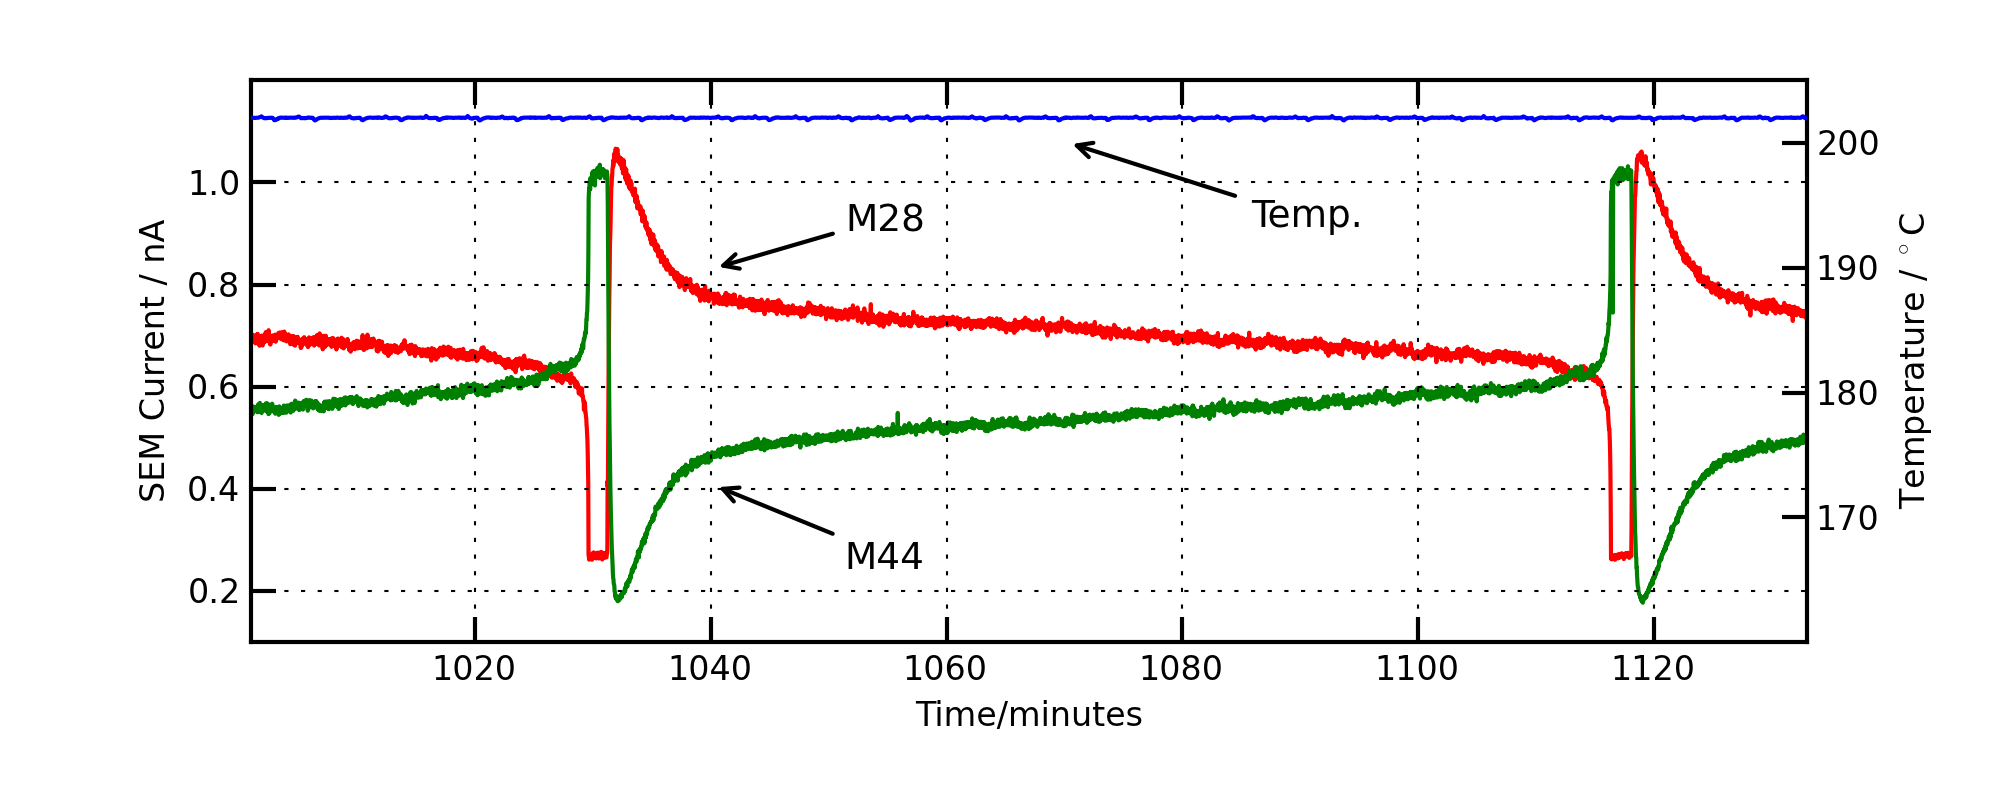
\includegraphics[width=17cm]{single_full_oscillation.png}
  \caption{A full oscillation period first showing a steep ignition of the sample followed by an almost immediate deactivation. For the next 65 minutes the sample slowly recovers activity until full conversion is reached again and the cycle repeats itself. This extremely long oscillation period is not commonly seen and was a result of careful parameter tuning. Typical oscillation periods are normally between $\sim$30\,s and $\sim$30\,min. Inserted circles illustrates the proposed model. At high conversion the platinum is oxidized (red) while in low conversion the sample is reduced (blue).}
  \label{fgr:full_oscillation}
\end{scheme}

After prolonged measurements over several days an increase in oscillation period was observed as shown in Figure \ref{fgr:long_measurement}. Initially, the oscillation period is $\sim$2.5 min and increases linearly with time until 1500 min of total oscillation time. Hereafter the oscillations become more irregular as shown in Figure~\ref{fgr:extracts} and lower panel Figure~\ref{fgr:long_measurement}. At experiment end the oscillation period is between 20 and 45 min.

\begin{scheme}
  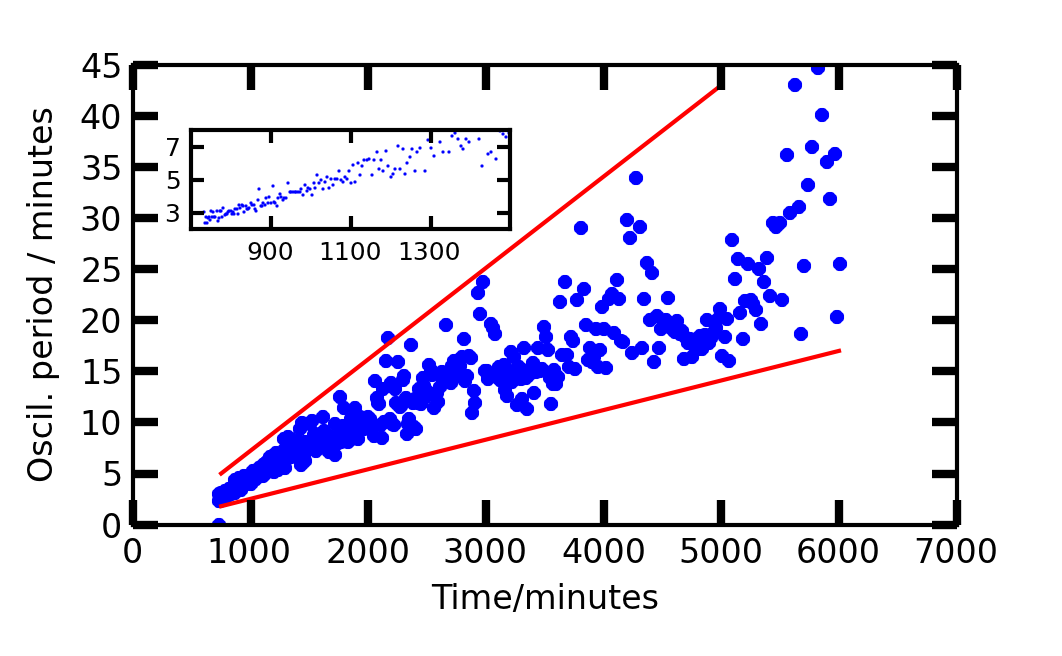
\includegraphics[width=9cm]{summary_of_long_measurement.png}
  \caption{Summary of the oscillation period as a function of time for a sample oscillating under constant temperature, pressure and reactant composition. The sample went through a total of 439 oscillations in 4 days. Time is defined from experiment start and hence includes initial treatment. The inset shows the initial steady increase in oscillation period.}
  \label{fgr:long_measurement}
\end{scheme}
  
Figure~\ref{fgr:extracts} shows extracts of mass spectrometry data of oscillations extracted from the same four days measurement. Data from shortly after the initial treatment, after 2800\,min of oscillation time and after 5900\,min are shown. After 5900\,min the oscillations are more irregular which is consistent with the data shown in Figure \ref{fgr:long_measurement}. Also, oscillations in between full conversion oscillations with smaller amplitude and much higher frequency than the full on-off cycles become more visible as time progresses.
\begin{scheme}
  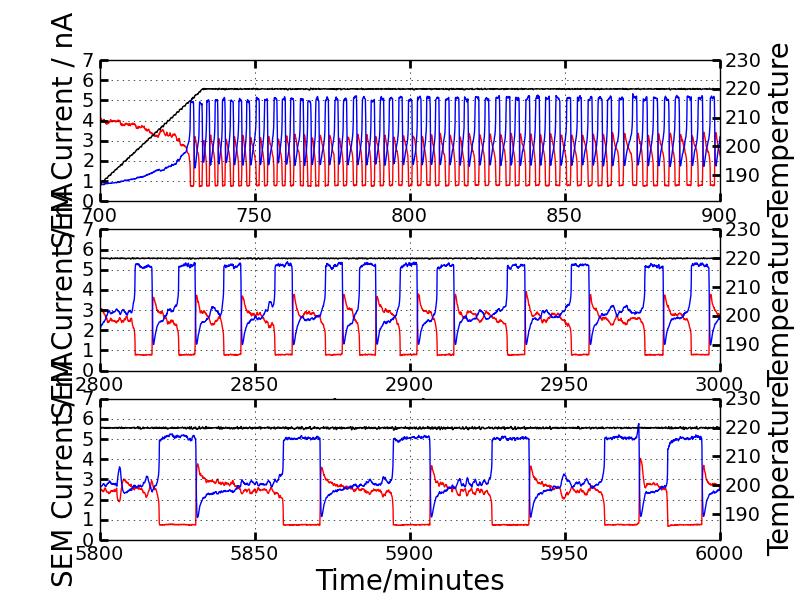
\includegraphics[width=9cm]{extracts_from_very_long_oscillation.png}
  \caption{Extracts from the 4 days long experiment. The oscillation period becomes more irregular with time while the total integrated conversion remains constant. Furthermore, small oscillations in between full conversion cycles become more prominent as time progresses.}
  \label{fgr:extracts}
\end{scheme}

The oscillation frequency becomes more irregular with progressing experiment time as shown in Figure \ref{fgr:extracts}. However, the ratio between CO and CO$_2$ integrated over an full period remains constant throughout the entire experiment time, i.e. the samples maintains a constant average rate independent of oscillation frequency. 

\begin{scheme}
  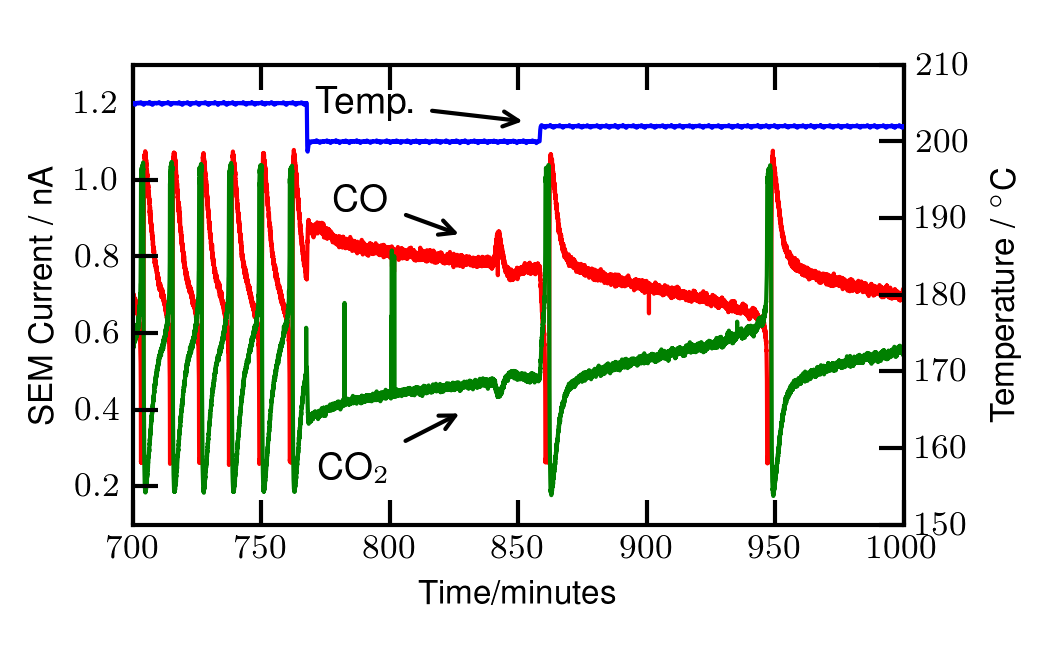
\includegraphics[width=9cm]{temperature_dependence.png}
  \caption{After about 10 hours of oscillations at 205$^\circ$C the temperature is first lowered by 5$^\circ$C and soon after increased by 2$^\circ$C. Before the temperature step the oscillation period was approximately 500\,s and after the step the period is approximately 5000\,s.}
  \label{fgr:temperature_dependence}
\end{scheme}

A very strong temperature dependence on the oscillation frequency was also found as shown in Figure~\ref{fgr:temperature_dependence}. By changing the temperature 5$^\circ$C the oscillation period was changed by more than a factor of 10. The magnitude of the change is not completely consistent across all measured samples but all samples show a very large temperature dependency where in some cases a provoked small change in temperature will consistently turn on and off the oscillations.

The pressure dependence of the oscillations was also investigated. In the pressure range of 0.1\,bar to 1\,bar no change of the oscillation frequency or qualitative behavior that could be attributed to the pressure was found. Similarly, only a weak dependence on the CO/O$_2$ ratio was observed. At a CO/O$_2$ ratio of $\sim0.025$ only very small amplitude oscillations was observed. Increasing the CO/O$_2$ showed clear oscillations with a significant increase in oscillation amplitude compared to lower CO concentrations. Generally, a tendency towards longer oscillation periods for higher CO/O$_2$ ratio was observed. Richer CO mixtures than 0.175 did not produce any oscillations in our system.

Although oscillations have previously been observed on extended Pt thin films \cite{Singh2010} as well as single crystals\cite{Hendriksen2005} at atmospheric pressure no oscillations could be provoked on thin films of comparable geometrical coverage to the nanoparticles in our system at any CO/O$_2$ ratio.  

%No consistent dependency on oscillation frequency and duty cycle was found that could be attributed to the size of the particles.

\subsection{CO concentration dependence}
The dependence of the CO concentration on the period of the oscillations was investigated. The result shows that the period increases slightly with increasing CO-concentration. However, the effect is small compared to the general trend of slower oscillations as the experiment progresses. In Figure~\ref{fgr:gas_dependence_summary} the oscillation periods are summarized and the actual masspectrometry data of the entire experiment is shown in Figure~\ref{fgr:gas_dependence}.

\begin{scheme}
  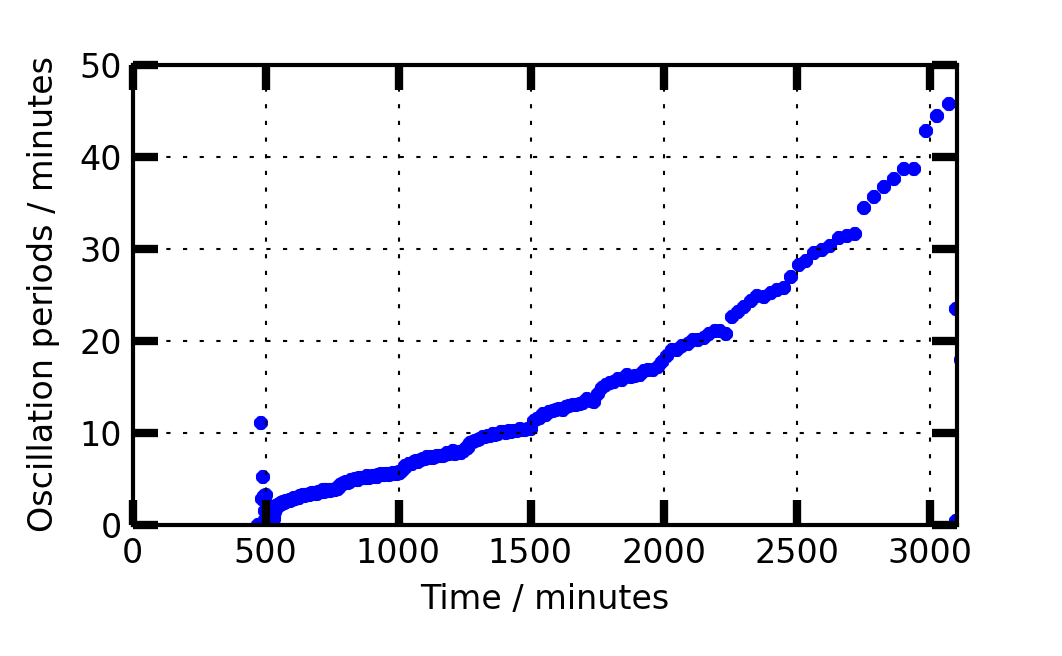
\includegraphics[width=9cm]{oscillations_gas_dependence_summary_supplemental.png}
  \caption{Summary of the gas-dependence. The overall trend of increasing oscillation period is now supporimposed by small discontinous stpes when the CO concentration is increased.}
  \label{fgr:gas_dependence_summary}
\end{scheme}

\begin{scheme}
  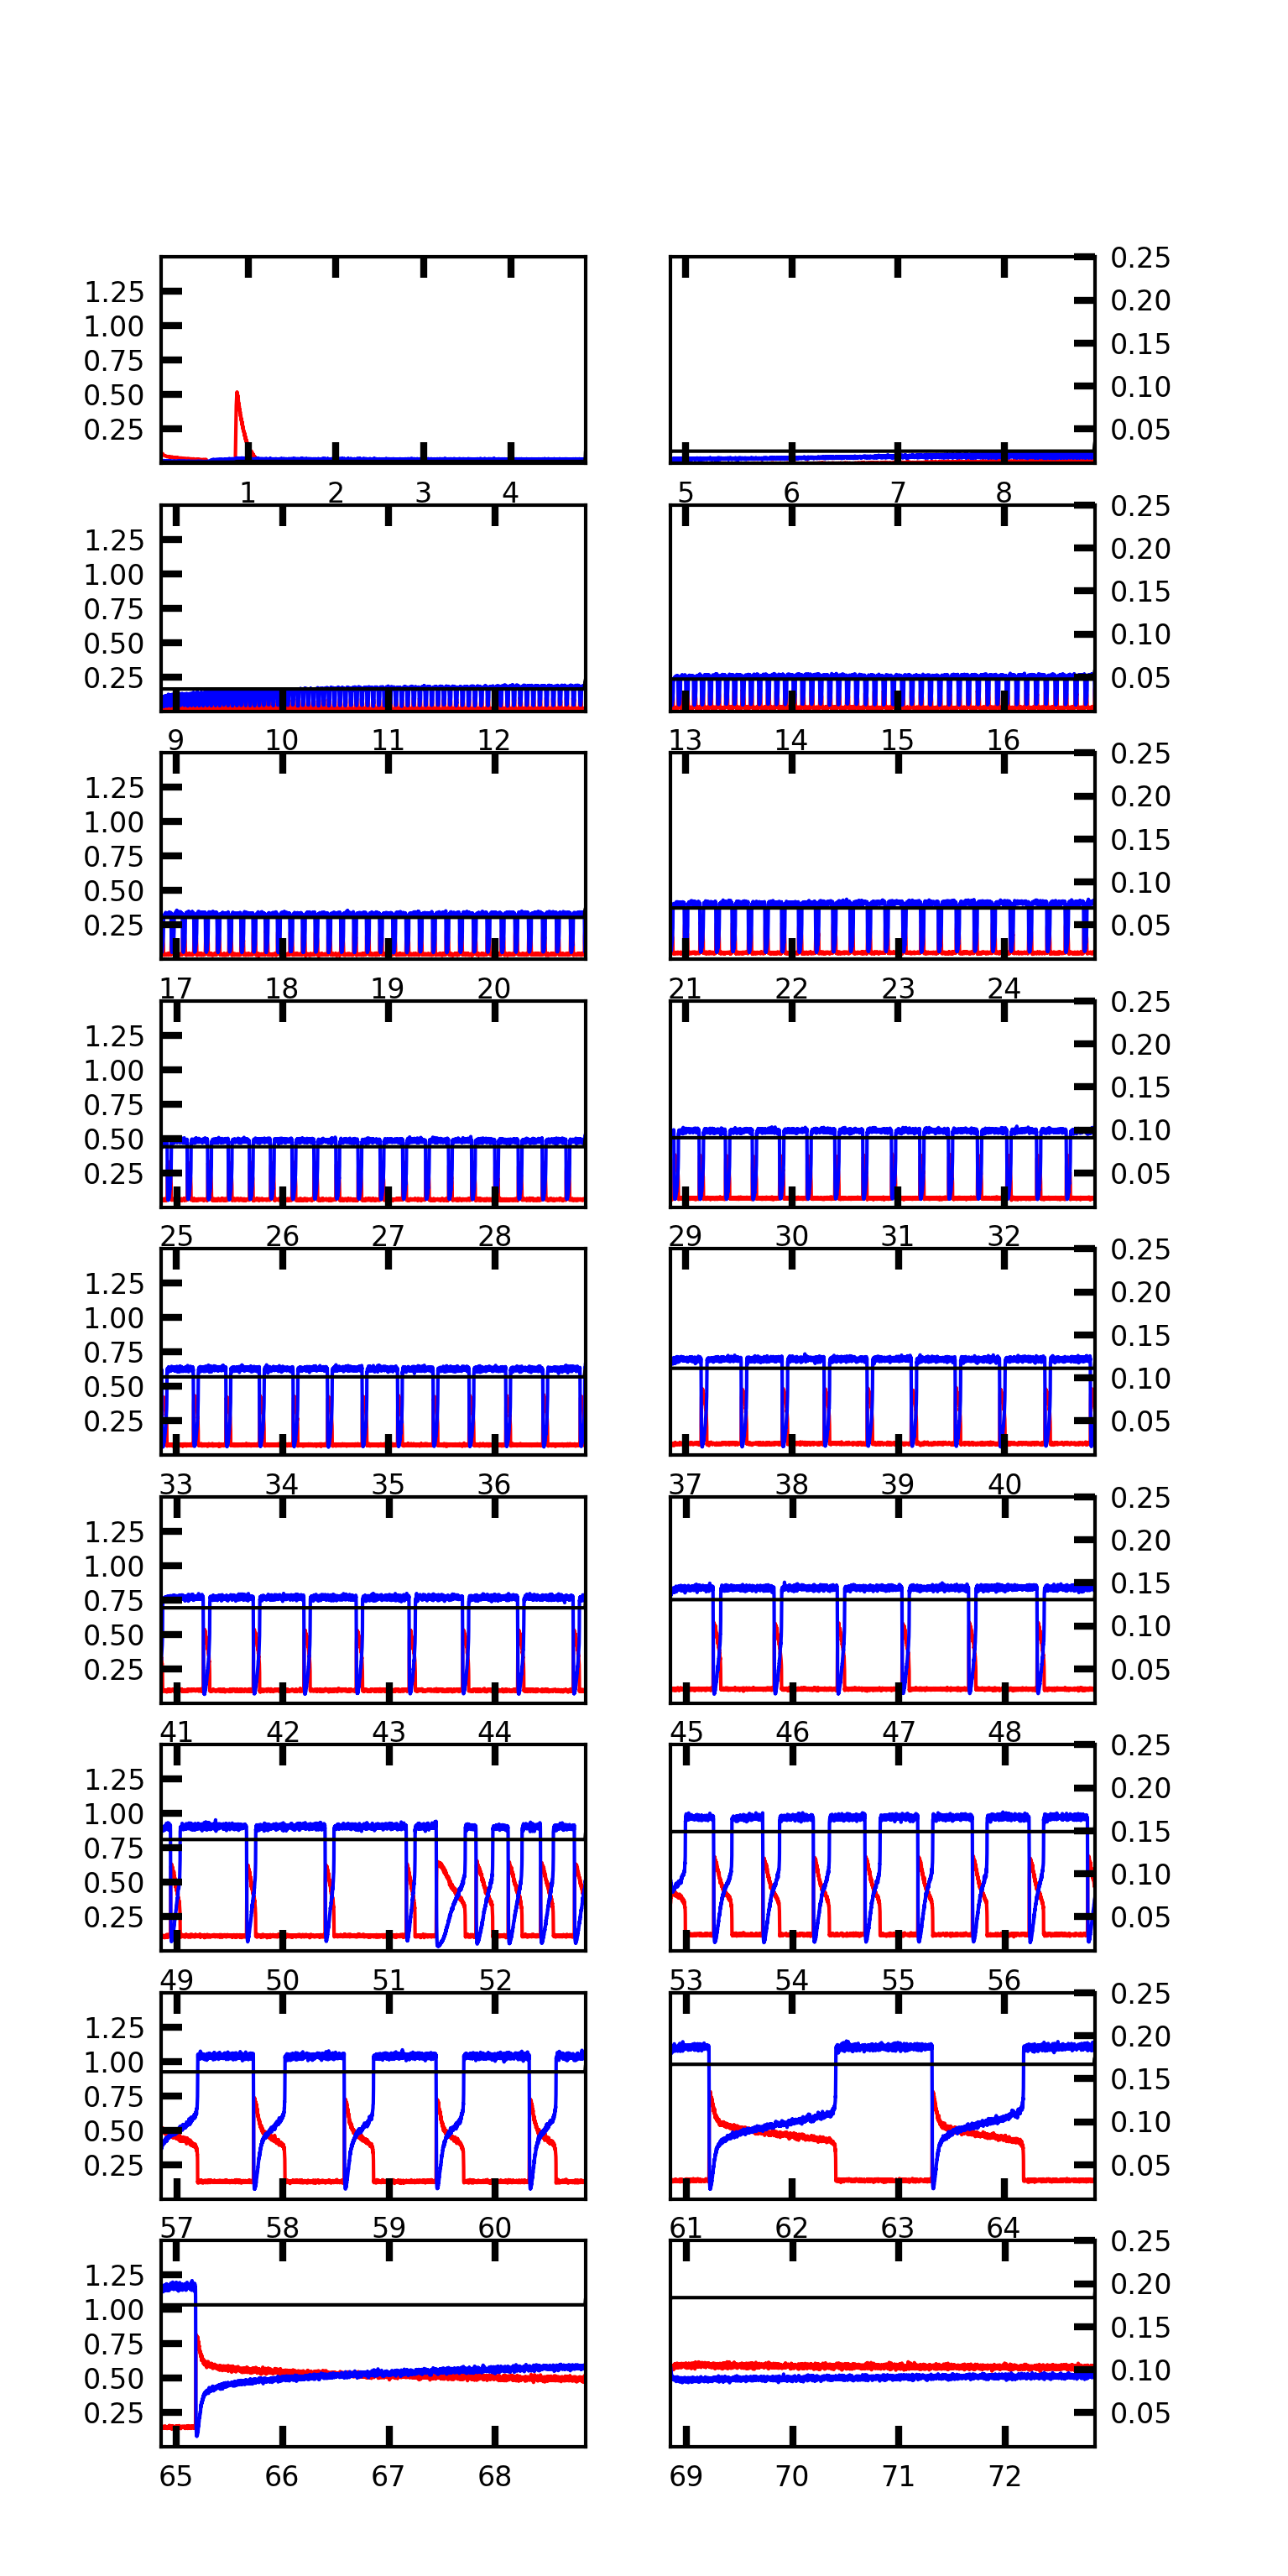
\includegraphics[width=14cm]{oscillations_gas_dependence_supplemental.png}
  \caption{Complete series of oscillating sample, showing CO (red) and CO$_2$ (blue). The temperature is constant $210^\circ$C doing the entire measurement. For every frame the CO-concentration is increased.}
  \label{fgr:gas_dependence}
\end{scheme}

\subsection{Temperature dependence}
As mentioned in the main paper, the oscillations shows a very strong temperature dependence. In Figure~\ref{fgr:temperature_dependence_supplemental} we show an example where the oscillations are turned on and off by changing the temperature $20^\circ$C.

\begin{scheme}
\centering
  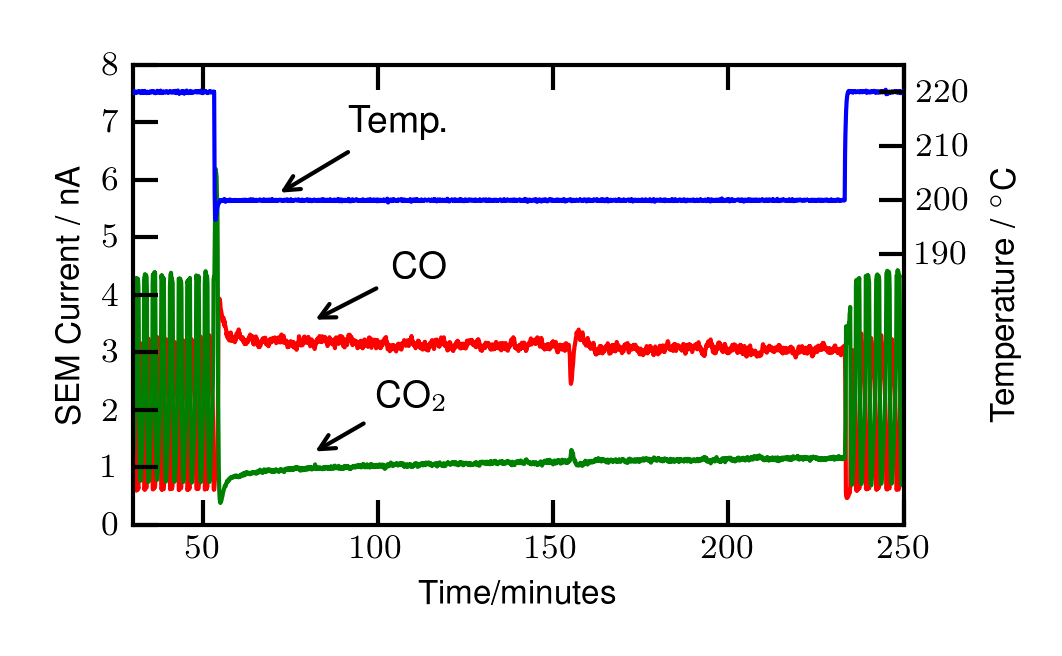
\includegraphics[width=9cm]{temperature_dependence_supplemental.png}
  \caption{Another example of the very pronounced temperature dependence.}
  \label{fgr:temperature_dependence_supplemental}
\end{scheme}

\subsection{Duty cycle}
Even though the period of the oscillations increases with time, the total integrated conversion rate during a complete cycle is almost constant. In Figure~\ref{fgr:duty_cycles_supplemental}, the value of the mean value of CO and CO$_2$ is plotted for every oscillation in the four-day long experiment. It is evident that the ratio between CO and CO$_2$ is almost constant and thus the average activity of the sample is almost unchanged despite the development in the oscillation frequency.


\begin{scheme}
  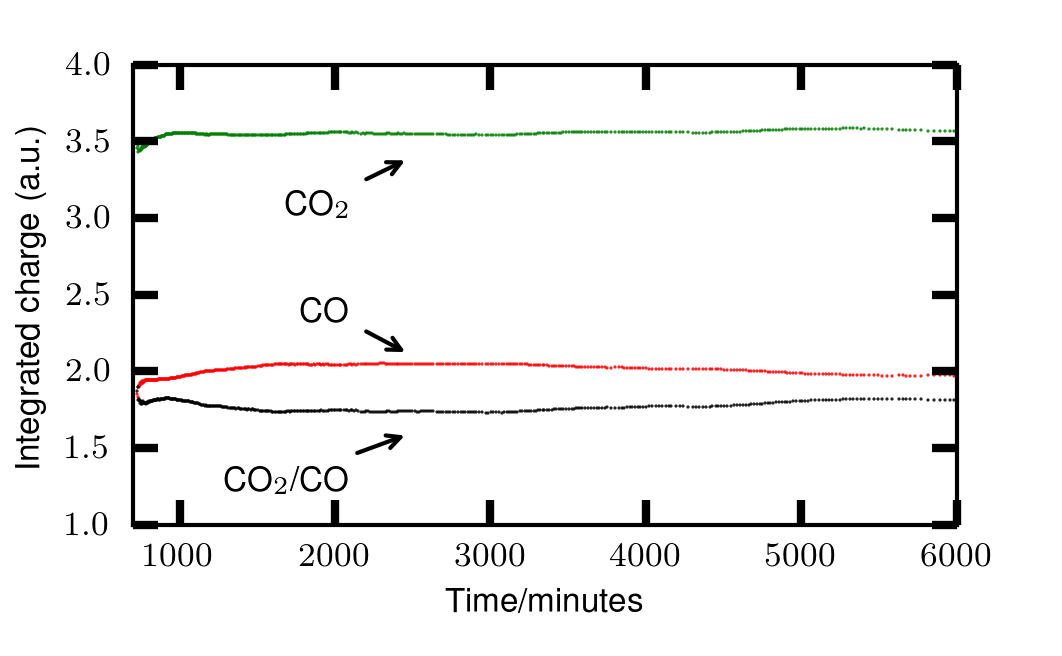
\includegraphics[width=9cm]{duty_cycles_long_measurement_supplemental.png}
  \caption{A plot of the duty-cycle of the sample duing the 4-day long experiment. The individual data-points is calculted as the integral of CO (red) or CO$_2$ (blue) doing the individual oscillations. The ratio between CO and CO$_2$ is drawn in black.}
  \label{fgr:duty_cycles_supplemental}
\end{scheme}


\section{Discussion}
Due to the long timescales between full conversion and low conversion plateaus the oscillations cannot be attributed to the reactor setup itself which due to its small size has timescales on the order of seconds. Furthermore, a series of experiments was performed to exclude the oscillations as an instrumental artifact. Firstly, experiments were performed on larger volume reactor thus increasing the residence time in the reactor. Secondly, the oscillations were reproduced on a comparable but not identical setup. Finally, attempts at reproducing the phenomenon on Pt-thin films of comparable coverage did not produce any oscillations. All of these experiments suggest that the oscillations is a property of the Pt nanoparticles.

It has previously been shown using STM \cite{Hendriksen2002}, FT-IR \cite{Carlsson2006}, Monte Carlo simulations \cite{Zhdanov2002} as well as DFT \cite{Gong2004} that the activity of Pt towards CO oxidation at atmospheric pressures is highly dependent on the oxidation state of the surface. A detailed proposal for the reaction mechanism on Pd has been developed by Hendriksen \textit{et. al.}\cite{Hendriksen2010} and our data is consistent with this model.

According to the proposed model in ref.~\citenum{Hendriksen2010} the bare metal surface is less active than the oxidized surface. Oscillations originate from a switch between an oxidized surface and the bare metal surface. Initially, with CO present in the inlet gas a smooth metal surface is exposed due to the general high adsorption energy of CO on metal surfaces. As the Pt nanoparticles convert the CO to CO$_2$ the partial pressure of CO will decrease and a Pt oxide will start to form in the high partial pressures of O$_2$ thus increasing the rate. The model\cite{Hendriksen2010} suggests that the oxidized nanoparticles will roughen during CO oxidation resulting in the formation of an increasingly rough oxide surface. As the oxide becomes rougher the bare metal surface is increasingly favored resulting in a return to the lower rate rough metal state. As the rate decreases the CO partial pressure increases which results in a transition from rough metal surface to a smooth metal surface. When the sample is sufficiently smooth it will again oxidize and thus complete the oscillation cycle. 

In this study Pt nanoparticles were investigated which, compared to a single crystal or a thin film, is a very rough surface. It is to be expected that the particles will initially favor the reduced state. As the reaction runs the gas composition towards the outlet of the reactor will become more oxidizing increasing the oxidation rate of the particles (illustrated in Figure~\ref{fgr:full_oscillation}). Gradually, as the particles toward the outlet oxidizes the turn-over will increase and the general CO concentration will decrease promoting more and more particles to oxidize which will gradually be seen in the QMS as an increase in CO$_2$ and a decrease in CO. As the CO concentration decreases the light-off temperature will decrease hence approaching the constant temperature of the sample resulting in a steep increase in reactivity. It is important to note that the fraction of oxidized particles needed to achieve full conversion is not known. We are currently investigating new methods for gaining insight into the nature of the nanoparticles in the reactor but the low coverage and the design of the reactor makes this a challenging task. If not all particles are oxidized at light-off they will now oxidize much faster due to the low CO-concentration. The further increased rate will not be visible in the QMS since the reactor is already in full conversion. As most of the particles are now oxidized they will become more and more roughened and gradually return to the reduced state. Fewer and fewer oxidized particles will be responsible for the activity increasing the roughing rate of the remaining active particles. Just before the overall activity drops only a fraction of the particles participates in the reaction and the deactivation will happen very suddenly. Once these potentially few particles eventually becomes sufficiently rough they will reduce and lose activity hence completing the oscillation cycle. It should be noted that our group has recently measured turnover frequencies of CO oxidation on Pt in excess of $10^{6}$s$^{-1}$ per site corresponding to as little as $\sim$300 Pt nanoparticles contributing to the reactivity just before the end of the high-activity cycle.

The oscillation period increases with time and becomes increasingly less stable as shown in Figure~\ref{fgr:extracts}. This phenomena is consistent across all measured samples. The large scatter in oscillation period can be attributed to the smaller oscillations in between on/off cycles. Occasionally, these small amplitude oscillations will trigger a full switch thus introducing more short-period oscillations despite the trend of increasingly slower oscillation period. A possible explanation of the phenomeonon could be sintering of the particles during the oxidation and reductions cycles. However, since the average conversion integrated over full oscillation periods is constant we do not expect sintering to be the cause since an average loss in activity of the sample would then be expected.

Oscillations were only seen in CO/O$_2$ ratio below 0.175. This ratio agrees well with literature \cite{Singh2010,Hendriksen2005} where oscillations have been observed in oxygen rich CO/O$_2$ mixtures. The needed low concentration of CO in the inlet gases can be attributed to the much higher sticking coefficient of CO on Pt which poisons the nanoparticle surface during the low reactivity region of the cycle. 

Nanoparticles of several different sizes were tested and all showed oscillations. However, no change in duty cycle or frequency that could be attributed to the size of the nanoparticles was found. This may be due to the fact that even nominally identical samples also show a large variation in oscillation frequency and duty cycle thus possibly shadowing a nanoparticle size effect.

An interesting feature in the data is the very large temperature dependence on oscillation frequency. This property agrees well an earlier suggested model \cite{Hendriksen2010} and it is, to our knowledge, the first time the temperature dependence of oscillations at atmospheric pressure has been measured.

\section{Conclusion}
Self-sustained CO oxidation oscillations at atmospheric pressure on Pt nanoparticles ranging from from 3\,nm to 9\,nm have been measured with high-quality mass-spectrometry. It was found that the samples increased the oscillation period over time and showed a strong temperature dependence. A model is proposed where the nanoparticles go through repetitive oxidation/reduction cycles which change the change rate of CO oxidation on the particles.

\bibliography{literature} %your .bib file


\end{document}
